\subsection{Diseño del experimento sobre el Rendimiento del\\ Sistema MOLDEAS}
El objetivo de un experimento es averiguar si unos determinados 
factores influyen en una determinada variable de interés para así poder cuantificar dicha influencia. En el caso 
de esta sección, la variable a estudiar es el rendimiento de las consultas \gls{SPARQL} contra el \textit{endpoint} utilizado, si bien 
no es el experimento principal de este documento ya que conllevaría la comparación con distintos proveedores de 
repositorios \gls{RDF}, si que ha surgido la necesidad de abordar esta cuestión por la latencia en las consultas. La metodología utilizada 
para el diseño del experimento es la repetición, en condiciones indistinguibles, con el objetivo de minimizar la variabilidad 
del mismo y que el error experimental sea lo más pequeño posible.

El tratamiento del rendimiento de las consultas permite estudiar si las mejoras introducidas decrementan 
el tiempo de ejecución de las mismas partiendo de un caso básico sin ninguna optimización y a continuación, a 
través de distintas repeticiones y la introducción de optimizaciones extraer aquel conjunto de mejoras que 
permiten extraer la influencia de las características incorporadas, seleccionando así la combinación con mejores resultados. Con este objetivo, 
se ejecutan las distintas iteraciones del experimento para a través de este proceso empírico detectar 
cambios significativos en la respuesta y comprender el comportamiento del rendimiento en las consultas. Por lo tanto, 
en este caso el experimento se realiza para encontrar las condiciones con las que se consigue la optimización 
más crítica y comparar las respuestas en tiempo de ejecución con la variación de las variables, \textit{a contrario sensu}, 
no es objetivo del experimento obtener un modelo matemático que permita realizar predicciones futuras. 

Un aspecto importante de este experimento es que la evaluación del mismo se realiza mediante los resultados obtenidos mediante 
una correcta planificación, esquivando el uso de datos históricos para no incurrir en errores debidos a la aleatoriedad. Por otra parte, 
durante la ejecución de un experimento suelen surgir distintos tipos de variabilidades que deben ser tomadas en cuenta:
\begin{itemize}
 \item Sistemática y planificada, cuyo origen viene determinada por las diferencias sistemáticas al modificar las condiciones, 
variables del experimento. Este tipo de variabilidad es conveniente y debe ocurrir para poder evaluar el experimento.
\item Debido a la naturaleza del problema y del experimento, se trata de variaciones debidas al ruido, error de medida, etc., siendo 
 impredecibles e inevitables. En el caso del experimento objeto de estudio se origina por cuestiones relacionadas con 
el tiempo de latencia en la red, etc. No obstante, esta variabilidad es medible y se puede extrapolar para la toma 
de decisiones.
\item Sistemática y no planificada, cuyo origen se debe a causas desconocidas, generando resultados sesgados. En el caso 
de estudio este tipo de variabilidad ha sido resuelta realizando las distintas réplicas en bloques de ejecución.
\end{itemize}

Una vez determinados los puntos clave a tener en cuenta para la evaluación de los resultados, es conveniente la caracterización 
propia del experimento que consta de las siguientes etapas:
\begin{enumerate}
 \item Definición de los objetivos del experimento. Las preguntas a responder por el experimento serán:
\begin{itemize}
 \item ¿Cuáles son las mejoras que se pueden aplicar sobre una consulta en SPARQL para mejorar el tiempo de ejecución?
 \item ¿Cuál es la combinación de mejoras que obtiene un mejor tiempo de respuesta?
 \item ¿Cuál es el coste de la combinación de estas mejoras? 
 \item ¿Existe algún elemento externo de configuración que implique un incremento en el tiempo de ejecución de las consultas? 
 \item ¿Cómo afectan los resultados en la implementación actual del sistema \gls{MOLDEAS}?
\end{itemize}
 \item Selección de una regla de asignación de las unidades experimentales a las condiciones de estudio. En este caso, 
la unidad experimental de este estudio será un repositorio RDF con un determinado orden de ejecución de cada uno 
de los tratamientos (variedad de consultas, casos de test $T_k$) para obtener las medidas de las observaciones, de esta forma se deben atender a los siguientes factores:
\begin{itemize}
 \item Cualitativos: tipo de entorno hardware y software, tipo de consulta en SPARQL con variaciones.
 \item Cuantitativos: tamaño de la muestra, de la memoria y número de réplicas.
\end{itemize}

En cuanto a la caracterización de los factores cualitativos, respecto al entorno hardware y software se utiliza el definido en la Sección~\ref{exp-general}. Sobre las consultas en SPARQL, existen trabajos sobre la optimización de las mismas~\cite{Schmidt2010,Bernstein07optarq:a,sparqlOpt} para la 
consulta eficiente de diferentes repositorios RDF~\cite{Yan:2008:EQR:1367497.1367652}, en este caso el tipo de consulta se centra en dos principales 
variables de información de los anuncios de licitación, los códigos CPV (tipo) y NUTS (localización), para ello tras la ejecución de método 
de expansión de conceptos a partir de un código inicial se obtienen una serie de códigos recomendados para su posterior transformación en una 
consulta en SPARQL, la lista completa de los códigos se presenta en la Tabla~\ref{tabla:queries}. Se debe destacar que el método de expansión 
es independiente de esta prueba ya que simplemente se necesitan códigos independientemente de su calidad y su descripción. La selección de códigos se ha llevado a 
cabo contemplando que los tipos presentes en el \gls{CPV} (División, Grupo, Clase y Categoría) estén representados ($Q_{1..8}$), 
además de proveer una consulta aleatoria $Q_9$, sobre los códigos \gls{NUTS} se han escogido aquellos representativos de países 
con el objetivo de generalizar y obtener un mayor número de resultados.

\begin{table}[!ht]
\renewcommand{\arraystretch}{1.3}
\begin{center}
\begin{tabular}{|p{3cm}|p{2.5cm}|p{3.5cm}|p{3.5cm}|}
\hline
  \textbf{ID Consulta} & \textbf{Código CPV inicial} & \textbf{Códigos CPV expandidos} & \textbf{Códigos NUTS}  \\ \hline
  $Q_1$ & 15331137 & 48611000, 48611000, 50531510, 15871210 & UK, PL, RO \\ \hline
  $Q_2$ & 50531510 & 34144100, 44212211, 44212212, 50531500 & ES, FR, DE \\ \hline
  $Q_3$ & 34144100 & 44212211, 31140000, 31140000, 34144100 & PL, CZ, RO \\ \hline
  $Q_4$ & 64122000 & 64216120, 79571000, 15871210, 64121000 & BE, SE, DE \\ \hline
  $Q_5$ & 79320000 & 75241000, 75100000, 75000000, 60112000 & UK, FR, AT \\ \hline
  $Q_6$ & 44100000 & 44110000, 44170000, 44190000, UB03 & NL, SE, DE \\ \hline
  $Q_7$ & 31000000 & 33141000, 39000000, 44000000, 31600000 & DE, IT, HU \\ \hline
  $Q_8$ & 50000000 & 50512000, 50333100, 50530000, 50532300 & UK, IR, FR \\ \hline
  $Q_9$ (random)   & 15841400 & 15841300, 15511700, 44921210, 03131400 & ES, FR, DK \\ \hline
  \hline
  \end{tabular}
  \caption{Descripción de los códigos en las consultas en SPARQL del experimento.}
  \label{tabla:queries}
  \end{center}
\end{table} 

En referencia a los aspectos cuantitativos del experimento, el tamaño de la muestra consta de nueve consultas ($Q_{1..9}$), el número de réplicas 
para evitar el ruido y la aleatoriedad previamente comentada es de $3$ y la situación de partida para cada una de ellas se produce 
bajo las mismas condiciones: reinicio de la máquina y consultas de entrenamiento (1 simple y 1 expandida) antes de la ejecución de una réplica para la obtención 
de las observaciones de tiempo de ejecución. Referente al tamaño de la muestra, se utilizará el \textit{endpoint} descrito anteriormente y con la carga 
de tripletas generada a partir de la aplicación de los métodos semánticos a los anuncios de licitación y siguiendo la distribución por 
grafos nombrados especificada en el Sección~\ref{sect:pscs-data-model}.

Por otra parte, las características, $F_i$, a evaluar en combinación se presentan en la siguiente Tabla~\ref{table:sparql-features}, en resumen se parte de una 
consulta simple (1 código CPV y 1 código NUTS) para obtener un tiempo de referencia, a partir de esta primera referencia se aplican 
las distintas optimizaciones, generando los distintos tratamientos ($T_i$), ver Tabla~\ref{tabla:tests}, para el establecimiento de la mejor combinación posible.

 \item Especificación de las medidas de trabajo en cuanto a la respuesta. El valor que se toma es el tiempo de ejecución 
en segundos de la consulta en SPARQL. 
 \item Ejecución de un experimento piloto. Evidentemente esta tarea se ha realizado con una pequeña muestra de consultas, sólo un año de anuncios 
de licitación pero ejecutando todos los tratamientos con el fin de validar el enfoque propuesto, obtener los resultados de toma de tiempos y preparar 
el procesamiento del registro de tiempos para obtener las medidas finales.
 \item Especificación de un modelo. En este caso, no se utilizará un modelo matemático para aproximar los valores, 
como ya se ha explicado anteriormente, debido a que el objetivo es optimizar la realización de consultas, en cuanto a 
tiempo de ejecución, no a la predicción futura.
 \item Esquematización de los pasos a seguir.
 \item Determinación del tamaño muestral. Como ya se ha comentado anteriormente, en el apartado de factores cuantitativos, se utilizarán los datos generados durante el proceso de promoción 
de datos a \linkeddata de los anuncios de licitación y de las clasificaciones de productos.
 \item Revisión de las decisiones anteriores.
\end{enumerate}

\newpage
\begin{longtable}[c]{|l|p{10cm}|} 
\hline
\textbf{ID} &  \textbf{Descripción}  \\\hline
\endhead
$F_1$ & Consulta simple: $1$ código CPV y $1$ código NUTS \\ \hline
$F_2$ & $F_1$ con uso de la claúsula \texttt{LIMIT} de SPARQL \\ \hline
$F_3$ & Consulta expandida: $n$ códigos CPV y $n$ código NUTS  \\ \hline
$F_4$ & Reescritura de las consultas SPARQL: \texttt{FILTER}, etc.  \\ \hline
$F_5$ & Uso de grafos nombrados en la consulta SPARQL: claúsula \texttt{FROM} \\ \hline
$F_6$ & Separación de las consultas en SPARQL en simples ($F_1$) \\ \hline
$F_7$ & Consultas simples distribuidas con $5$ hilos (1 por código CPV) \\ \hline
\hline
\caption{Características de las consultas en SPARQL.}\label{table:sparql-features}\\    
\end{longtable}


\begin{table}[!htb]
\renewcommand{\arraystretch}{1.3}
\begin{center}
\begin{tabular}{|p{3.5cm}|p{0.8cm}|p{0.8cm}|p{0.8cm}|p{0.8cm}|p{0.8cm}|p{0.8cm}|p{0.8cm}|p{2cm}|}
\hline
  \textbf{Test}/ \textbf{Característica}& \textbf{$F_1$} & \textbf{$F_2$} & \textbf{$F_3$} & \textbf{$F_4$} & \textbf{$F_5$} & \textbf{$F_6$} &  \textbf{$F_7$} & \textbf{Nº consultas SPARQL} \\ \hline
   $T_1$ & $\star$ & & & & & & &$1$\\ \hline 
   $T_2$ & $\star$ & & $\star$ & & & & &$1$\\ \hline 
   $T_3$ &  & $\star$ &  & & & & &$1$\\ \hline 
   $T_4$ &  & $\star$ & $\star$ & & & & &$1$\\ \hline 
   $T_5$ &  & $\star$ & $\star$ & $\star$ & & & &$1$\\ \hline 
   $T^{1}_6$ ($n$ códigos CPV y $m$ códigos NUTS)&  & $\star$ & $\star$ & $\star$ & $\star$ & $\star$ & &$4$\\ \hline 
   $T^{2}_6$ ($\equiv$)&  & $\star$ & $\star$ & $\star$ & $\star$ & $\star$ & $\star$ &$4$\\ \hline 
   $T^{1}_7$ ($1$ código CPV y $m$ códigos NUTS) &  & $\star$ & $\star$ & $\star$ &  & $\star$ &  &$5$ \\ \hline 
   $T^{2}_7$ ($\equiv$) & & $\star$ & $\star$ & $\star$ &  & $\star$ & $\star$ &$5$\\ \hline 
   $T^{1}_8$ ($\equiv$)& & $\star$ & $\star$ & $\star$ & $\star$ & $\star$ &  &$20$\\ \hline 
   $T^{2}_8$ ($\equiv$) & & $\star$ & $\star$ & $\star$ & $\star$ & $\star$ &  $\star$ &$20$\\ \hline 
   $T^{1}_9$ ($1$ código CPV y $1$ código NUTS ) & & $\star$ & $\star$ & $\star$ &  & $\star$ & &$15$  \\ \hline 
   $T^{2}_9$ ($\equiv$)& & $\star$ & $\star$ & $\star$ & & $\star$ &  $\star$ &$15$\\ \hline 
   $T^{1}_{10}$ ($\equiv$) & & $\star$ & $\star$ & $\star$ & $\star$ & $\star$ & &$60$  \\ \hline 
   $T^{2}_{10}$ ($\equiv$) & & $\star$ & $\star$ & $\star$ & $\star$ & $\star$ & $\star$ &$60$ \\ \hline 
  \hline
  \end{tabular}
  \caption{Descripción de cada uno de los tratamientos, características de optimización.}
  \label{tabla:tests}
  \end{center}
\end{table} 
\clearpage
\subsection{Ejecución del experimento sobre el Rendimiento del\\ Sistema MOLDEAS}
La aplicación del plan previsto en la anterior sección arroja un conjunto de valores para cada uno de los tratamientos ($T_k$) y réplicas de los tiempos 
de ejecución de las consultas, de acuerdo a las distintas características ($F_i$). En la Tabla~\ref{tabla:tests-agregado} se reflejan 
las medias de tiempo y ganancia agregadas de cada uno de los tratamientos realizados. Por otra parte, se presentan igualmente 
las medidas pormenorizadas de las observaciones realizadas y agregadas de las 3 réplicas ejecutadas, ver Tablas~\ref{tabla:results-1} y~\ref{tabla:results-2}. 
El cálculo de la ganancia se realiza mediante la fórmula: $t_{old}/t_{new}-1*100$, tomando como referencia para $T_2$, el tiempo de $T_1$ y para 
los tratamientos $T_{4..10}$, el tiempo de $T_3$. Finalmente, la ejecución de todos los tratamientos con las distintas observaciones y 
réplicas ha implicado la realización de $5751$ consultas en SPARQL, más las de entrenamiento para cada una de las réplicas. 

\begin{table}[!htb]
\renewcommand{\arraystretch}{1.3}
\begin{center}
\begin{tabular}{|l|c|c|}
\hline
  \textbf{Test}& \textbf{$\bar{X}$ Tiempo (seg.)} & \textbf{$\bar{X}$ Ganancia (\%)} \\ \hline
   $T_1$ & $3.21$  & N/A\\ \hline 
   $T_2$ & $3.25$  & $1.21$   \\ \hline 
   $T_3$ & $20.548$ & N/A   \\ \hline 
   $T_4$ & $20.552$ & $-0.02$ \\ \hline 
   $T_5$ & $20.545$ & $-0.01$ \\ \hline 
   $T^{1}_6$ & $20.52$  & $0.14$\\ \hline 
   $T^{2}_6$ & $11.80$ & $74.37$\\ \hline 
   $T^{1}_7$ & $15.81$ & $30.58$ \\ \hline 
   \textbf{$T^{2}_7$} & \textbf{$10.51$} & \textbf{$96.54$} \\ \hline
   $T^{1}_8$ & $32.33$ & $-36.11$ \\ \hline 
   $T^{2}_8$ & $18.45$ & $11.21$ \\ \hline 
   $T^{1}_9$ & $22.53$ & $-8.77$ \\ \hline 
   $T^{2}_9$ & $12.61$ & $63.36$ \\ \hline 
   \textbf{$T^{1}_{10}$} & \textbf{$71.01$} & $-70.97$ \\ \hline 
   $T^{2}_{10}$ & $35.08$ & $-40.42$ \\ \hline 
  \hline
  \end{tabular}
  \caption{Tiempo de ejecución (seg.) y ganancia (\%).}
  \label{tabla:tests-agregado}
  \end{center}
\end{table} 



\begin{table}[!h]
\renewcommand{\arraystretch}{1.3}
\begin{center}
\begin{tabular}{|p{1.5cm}|p{1.5cm}|p{1.5cm}|p{1.5cm}|p{1.5cm}|p{1.5cm}|p{1.5cm}|p{1.5cm}|}
\hline
\textbf{ID Consulta/ Test} & $T_1$ & $T_2$ & $T_3$ & $T_4$ & $T_5$ & $T^{1}_{6}$ & $T^{2}_{6}$ \\ \hline
  $Q_1$ & $3.21$ (NA) & $3.13$ ($2.46$) & $19.35$ (NA) & $19.53$ ($-0.91$) & $19.45$ ($0.49$)  & $19.24$ ($0.58$) & $11.16$ ($73.49$)\\ \hline
  $Q_2$ & $3.15$ (NA) & $3.14$ ($0.52$) & $23.56$ (NA)   & $23.68$ ($-0.52$)  & $23.68$ ($0.52$) & $24.06$ ($-2.10$) & $13.24$ ($77.95$) \\ \hline
  $Q_3$ & $3.14$ (NA)  & $3.14$ ($0.11$) & $18.56$ (NA)  & $18.47$ ($0.46$)  & $18.44$ ($-0.60$)  & $18.69$ ($-0.71$)  & $10.08$ ($84.14$) \\ \hline
  $Q_4$ & $3.16$ (NA)  & $3.13$ ($0.79$) & $18.52$ (NA)  & $18.32$ ($1.08$)  & $18.50$ ($-0.10$)  & $18.20$ ($1.77$)  & $10.19$ ($81.73$) \\ \hline
  $Q_5$ & $3.29$ (NA)  & $3.17$ ($3.82$) & $22.69$ (NA)  & $22.85$ ($-0.72$)  & $22.69$ ($0.01$)  & $22.62$ ($0.31$)  & $14.61$ ($55.31$) \\ \hline
  $Q_6$ & $3.21$ (NA)  & $3.17$ ($1.35$) & $18.55$ (NA)  & $18.45$ ($0.51$)  & $18.48$ ($-0.35$)  & $18.22$ ($1.78$)  & $10.00$ ($85.46$) \\ \hline
  $Q_7$ & $3.39$ (NA)  & $3.39$ ($0.25$) & $19.01$ (NA)  & $19.19$ ($-0.93$)  & $19.12$ ($0.55$)  & $18.99$ ($0.09$)  & $11.08$ ($71.56$) \\ \hline
  $Q_8$ & $3.94$ (NA)  & $3.98$ ($-0.95$)& $23.44$ (NA)  & $23.15$ ($1.26$)  & $23.24$ ($-0.82$)  & $23.50$ ($-0.29$)  & $14.72$ ($59.24$) \\ \hline
  $Q_9$ & $3.17$ (NA)  & $3.09$ ($2.59$) & $22.23$ (NA)  & $22.32$ ($-0.40$)  & $22.27$ ($0.19$)  & $22.26$ ($-0.15$)  & $12.32$ ($80.45$) \\ \hline
  \hline
  \end{tabular}
  \caption{Tiempo de ejecución (seg.) y ganancia (\%). Parte 1.}
  \label{tabla:results-1}
  \end{center}
\end{table} 


\begin{sidewaystable}[ht!]
\renewcommand{\arraystretch}{1.3}
\begin{center}
\begin{tabular}{|p{1.5cm}|p{1.5cm}|p{1.5cm}|p{1.5cm}|p{1.5cm}|p{1.5cm}|p{1.5cm}|p{1.5cm}|p{1.5cm}|p{1.5cm}|}
\hline
\textbf{ID Consulta/ Test} & $T^{1}_{7}$ & $T^{2}_{7}$ & $T^{1}_{8}$ & $T^{2}_{8}$ & $T^{1}_{9}$ & $T^{2}_{9}$ & $T^{1}_{10}$ & $T^{2}_{10}$\\ \hline
  $Q_1$ & $15.71$ ($23.18$)  & $10.62$ ($82.25$) & $33.27$ ($-41.84$) & $18.75$ ($3.24$) & $21.58$ ($-10.33$) & $12.38$ ($56.28$) & $69.13$ ($-72.00$) & $33.41$ ($-42.07$) \\ \hline
  $Q_2$ & $15.64$ ($50.57$)  & $9.90$ ($137.84$) & $32.26$ ($-26.98$) & $17.96$ ($25.66$ ) & $26.27$ ($-10.34$) & $15.50$ ($51.97$) & $73.62$ ($-68.00$) & $37.50$ ($-29.49$) \\ \hline
  $Q_3$ & $15.54$ ($19.44$)  & $9.66$ ($92.13$ ) & $32.04$ ($-42.09$) & $17.94$ ($3.29$) & $20.32$ ($-8.68$) & $10.44$ ($77.68$) & $68.95$ ($-73.09$ ) & $32.95$ ($-50.52$) \\ \hline
  $Q_4$ & $15.87$ ($16.68$)  & $9.99$ ($85.45$) & $32.07$ ($-42.24$) & $18.43$ ($3.24$) & $20.48$ ($-9.54$) & $10.33$ ($79.23$) & $68.85$ ($-73.10$) & $34.27$ ($-43.79$) \\ \hline
  $Q_5$ & $16.18$ ($40.22$)  & $11.92$ ($90.39$) & $32.46$ ($-30.10$) & $19.02$ ($23.12$) & $24.28$ ($-6.57$) & $14.40$ ($57.55$) & $74.02$ ($-69.35$ ) & $37.08$ ($-33.79$) \\ \hline
  $Q_6$ & $15.76$ ($17.73$)  & $9.60$ ($93.21$) & $32.11$ ($-42.23$) & $18.24$ ($-2.48$) & $20.51$ ($-9.55$) & $10.77$ ($72.23$) & $72.28$ ($-74.34$ ) & $32.80$ ($-49.98$) \\ \hline
  $Q_7$ & $15.93$ ($19.31$)  & $11.23$ ($69.35$ ) & $32.21$ ($-40.99$) & $18.51$ ($4.23$) & $21.12$ ($-10.01$) & $11.27$ ($68.67$) & $69.02$ ($-72.46$) & $33.55$ ($-42.04$) \\ \hline
  $Q_8$ & $16.12$ ($45.43$)  & $12.11$ ($93.54$ ) & $32.55$ ($-28.01$) & $19.50$ ($26.61$) & $25.33$ ($-7.48$) & $16.16$ ($45.05$) & $72.72$ ($-67.77$) & $38.27$ ($-30.16$) \\ \hline
  $Q_9$ & $15.58$ ($42.66$)  & $9.89$ ($124.71$) & $31.99$ ($-30.51$) & $17.74$ ($14.01$) & $23.76$ ($-6.46$) & $13.76$ ($61.57$) & $70.76$ ($-68.59$) & $36.40$ ($-41.92$) \\ \hline
  \hline
  \end{tabular}
  \caption{Tiempo de ejecución (seg.) y ganancia (\%). Parte 2.}
  \label{tabla:results-2}
  \end{center}
\end{sidewaystable} 


Adicionalmente, los resultados agregados de este experimento, respecto a los tratamientos de referencia $T_1$ y $T_3$, 
se visualizan en las siguientes gráficas, ver Figuras~\ref{fig:results-graph-1} y~\ref{fig:results-graph-2} 
tomando como referencia el tiempo de ejecución y en la Figura~\ref{fig:results-graph-3} presentando la ganancia en porcentaje respecto a $T_3$.

\begin{figure}[!htb]
\centering
	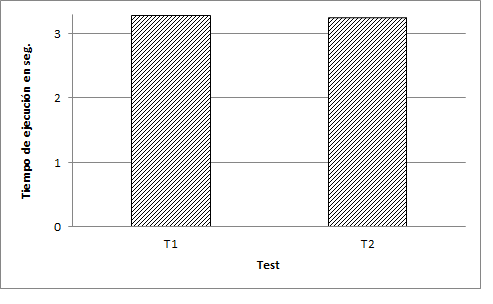
\includegraphics[width=12cm]{./images/phd/experimentation/t1-t2-tiempo}
\caption{Gráfica de Tiempo de ejecución medio con referencia $T_1$.}
\label{fig:results-graph-1}
\end{figure}

\begin{figure}[!htb]
\centering
	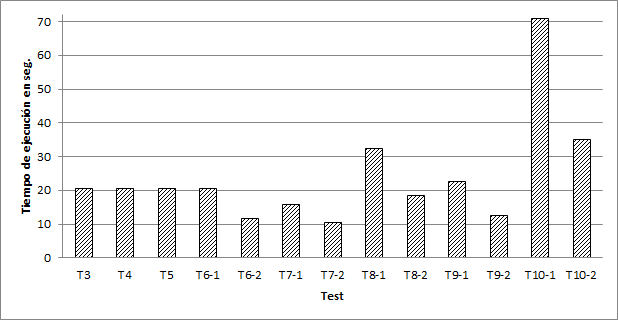
\includegraphics[width=14cm]{./images/phd/experimentation/t3-t10-tiempo}
\caption{Gráfica de Tiempo de ejecución medio con referencia $T_3$.}
\label{fig:results-graph-2}
\end{figure}

\begin{figure}[!htb]
\centering
	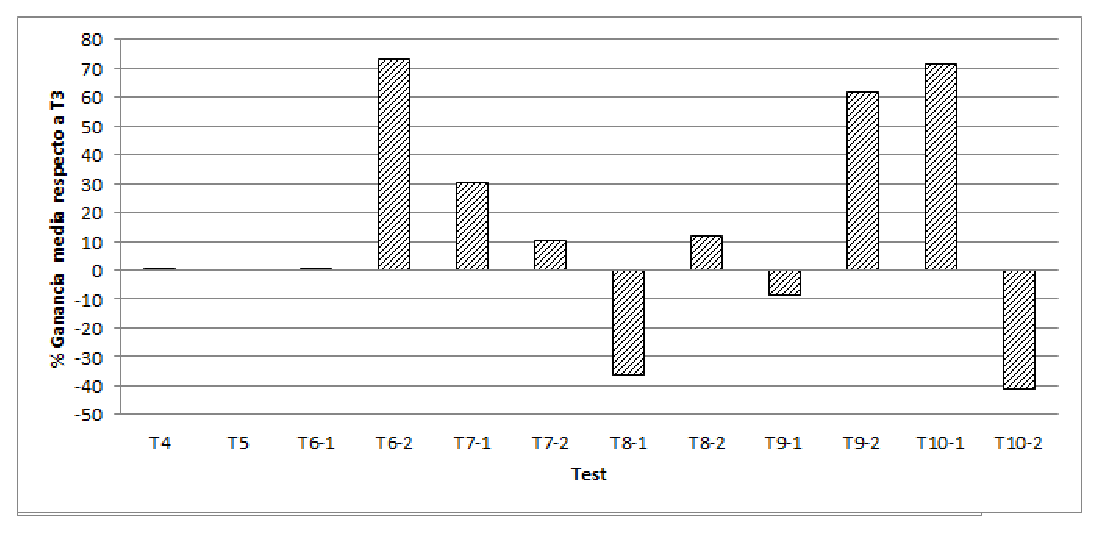
\includegraphics[width=14cm]{./images/phd/experimentation/t3-t10-ganancia}
\caption{Gráfica de Ganancia media con referencia $T_3$ en (\%).}
\label{fig:results-graph-3}
\end{figure}

\clearpage
\subsection{Validación del experimento sobre el Rendimiento del\\ Sistema MOLDEAS}
La realización del experimento de rendimiento de las consultas en \gls{SPARQL} es motivado por el exceso 
de latencia en las consultas al repositorio \gls{RDF}. Como ya se ha mencionado no es objetivo la comparación 
de distintos repositorios RDF para comprobar cuál obtiene un mejor rendimiento para las consultas realizadas, 
sino probar cuáles son las optimizaciones en las consultas en SPARQL y en el código fuente del demostrador que 
permiten acelerar el tiempo de la consulta independientemente del proveedor del servicio. Por ello, las características 
a combinar $F_i$, para obtener un mejor tiempo de respuesta permiten establecer la mejor conjunción de las mismas de acuerdo 
al estudio de los tiempos de ejecución obtenidos. 

De acuerdo a los resultados obtenidos se establecen los siguientes puntos clave y conclusiones:
\begin{itemize}
\item Los tipos de consulta generados a partir de $F_1$ y $F_3$ permiten establecer un valor de referencia 
en tiempo de ejecución para su posterior comparación con las mejoras introducidas. De esta manera se establece 
un primer valor de referencia para la comparación de consultas simples ($1$ código CPV y $1$ código NUTS) en torno 
a los $3$ segundos y otro para consultas expandidas, $n$ códigos CPV y $n$ código NUTS, en torno a los $20$ segundos. Estos 
valores son por una parte motivadores del experimento de mejora y por otra permiten evidenciar la ganancia con la introducción 
de nuevas características 
 \item Existen algunas de las características, $F_2$ y $F_4$, que no implican mejora en el tiempo de ejecución. 
\item En el caso particular de $F_3$, uso de la claúsula LIMIT, su valor se fija en $10000$ y carece de representatividad debido a que los resultados 
de la consulta ya son previamente filtrados y no superan esta cifra.
\item La reescritura de consultas, $F_4$, habitualmente implica mejoras en el tiempo de ejecución pero no se ha apreciado una mejora 
crítica debido a que este tipo de optimizaciones obtienen una mejora crítica cuando las consultas en SPARQL realizan operaciones 
con valores opcionales, claúsula OPTIONAL, por ejemplo cuando se trasladan consultas del tipo NATURAL JOIN e INNER JOIN en SQL a SPARQL, en el 
caso de estudio estos valores no se han utilizado ya que las consultas generadas por el sistema no incluyen encaje de patrones 
mediante claúsulas opcionales.
\item En cuanto a la característica $F_5$ sobre el uso de grafos nombrados se obtiene una mejora relevante, ya que la selección 
de los grafos sobre los cuales se realizan las consultas permite acotar el número de tripletas, no es lo mismo realizar sobre el 
grafo RDF completo presente en el \textit{endpoint} que sobre un subconjunto del mismo. Sin embargo, hay que destacar que la 
ejecución de múltiples consultas (separando por grafo) provoca que el tiempo de ejecución sea incrementado.
\item Sin duda la mejora más intensa en cuanto a tiempo de ejecución se produce en los casos $F_6$ y $F_7$ como se puede 
ver en los tratamientos $T^{2}_6$, $T^{1}_7$, $T^{2}_7$ y $T^{2}_9$, ya que el tiempo de ejecución de consultas simples 
es relativamente bajo y, evidentemente, la distribución de consultas permite la obtención de un mejor tiempo de ejecución 
global. No obstante, en los tratamientos $T^{1}_{10}$ and $T^{2}_{10}$ esta supuesta mejora se convierte en un inconveniente, 
ya que el número de consultas generadas es muy alto y la distribución mediante $5$ hilos no permite realizar una mejora.
\item Teniendo en cuenta los puntos anteriores cabe destacar que el tipo de códigos CPV no tiene ninguna implicación para 
la ejecución de la consulta. Sin embargo, el número de códigos \gls{CPV} sí implica un incremento en el tiempo de ejecución, del orden 
de $3$ segundos adicionales por cada código CPV nuevo, en cambio el uso de varios códigos NUTS no supone un incremento en el tiempo 
de ejecución y en el experimento la ejecución de un código CPV con varios \gls{NUTS} es similar a la combinación $n-m$ de los mismos.
\end{itemize}

A la vista de las conclusiones extraídas y de los resultados obtenidos se comprueba que la mejor combinación de características se 
genera en el tratamiento $T^{2}_7$, con un tiempo de ejecución de $10.55$ segundos y una ganancia respecto a $T_3$ del $95.73 \%$, la descripción 
de esta mejora implica que se trata de una consulta expandida ($F_3$), en la cual se utilizan claúsulas LIMIT ($F_2$), se reescriben 
las consultas mediante FILTERs ($F_4$), generando consultas simples en SPARQL ($F_6$) de 1 código CPV y $m$ códigos NUTS y, finalmente, 
se distribuyen con un hilo por código CPV. Por otra parte, el peor resultado se genera en el tratamiento $T^{1}_{10}$ con un tiempo de 
ejecución de $71.63$ segundos y una pérdida en ganancia del $-71.17 \%$, esta situación se debe a la extrema generación de consultas 
simples que si bien son rápidas en tiempo de ejecución por separado, el gran número de las mismas generadas implica que la supuesta 
ganancia se convierta en pérdida.

\subsection{Evaluación del experimento sobre el Rendimiento del\\ Sistema MOLDEAS}
La ejecución y validación del experimento mediante la extracción de una serie de conclusiones permiten 
dar respuesta las preguntas establecidas en el diseño del experimento.
\begin{itemize}
  \item ¿Cuáles son las mejoras que se pueden aplicar sobre una consulta en \gls{SPARQL} para mejorar el tiempo de ejecución? 

Existen diversas mejoras aplicables a las consultas en SPARQL dependiendo del tipo de encaje de tripletas que se realice, como el 
uso de la claúsula LIMIT, FILTER o los grafos nombrados, siendo independientes del proveedor del \textit{endpoint}. No obstante, estas 
mejoras no siempre son relevantes para todos los casos y en el caso particular estudiado su relevancia no es tan crítica 
como la separación de la consulta expandida en simples y su distribución.

 \item ¿Cuál es la combinación de mejoras que obtiene un mejor tiempo de respuesta? 

En el caso particular estudiado las características 
del tratamiento $T^{2}_7$ generan el mejor tiempo de ejecución utilizando consultas simples, con uso de claúsulas LIMIT y FILTER en SPARQL 
y distribuyendo la ejecución de las mismas.
 \item ¿Cuál es el coste de la combinación de estas mejoras? 

La generación de consultas a partir de una consulta expandida es un proceso 
trivial que no genera sobrecarga en tiempo de ejecución en el código. El esfuerzo recae sobre la programación distribuida con hilos, pero 
teniendo en cuenta las capacidades que suministran los lenguajes de programación actuales (Java) este tipo de práctica queda minimizada. Por tanto, 
el coste de implantación de esta solución es bajo.
 \item ¿Existe algún elemento externo de configuración que implique un incremento en el tiempo de ejecución de las consultas? 

El incremento del tiempo de ejecución se puede abordar desde dos puntos de vista: 1) el nuevo código fuente implica una lógica con una alta 
complejidad temporal, como se ha señalado la generación de consultas simples no resulta crítico y la programación distribuida, con su intrínseca 
dificultad, queda minimizada debido a las facilidades de los lenguajes de programación, en este caso Java y 2) el cambio del número de peticiones 
y consultas implica una sobrecarga en la red, conllevando un exceso en el tiempo de ejecución. En este caso, esta situación es minimizada 
tratándose de un entorno local y en el caso de un entorno global la situación tampoco se considera crítica debido a que las consultas 
están limitadas en tamaño y se facilitaría algún sistema de caché de consultas y resultados~\cite{Blanco:2010:CSE:1835449.1835466}.


 \item ¿Cómo afectan los resultados en la implementación actual del sistema \gls{MOLDEAS}?

La realización de este experimento ya ha generado una refactorización en el código del componente \textit{moldeas-api} para atacar 
la división de consultas expandidas en simples y la ejecución paralela de consultas, por lo que realmente este experimento 
ha servido para mejorar el tiempo de ejecución del sistema y el código fuente del mismo. Sobre la configuración necesaria 
para adoptar esta solución, el uso del \textit{framework} Spring facilita los cambios en las implementaciones de un interfaz, por lo que,
la dificultad para integrar nuevas implementaciones está minimizado con el uso de este tipo de tecnología.
\end{itemize}

Finalmente y como síntesis de esta sección cabe destacar que la ejecución de consultas sobre conjuntos de datos de cierta 
envergadura conlleva la aparición de problemas de escalabilidad y rendimiento que están siendo abordados en la comunidad 
de \linkeddata mediante la aplicación de técnicas distribuidas, igualmente es conveniente la realización de un esfuerzo 
para que las consultas en \gls{SPARQL} no supongan un cuello de botella en las aplicaciones que hagan uso de tecnologías 
semánticas, para ello los estudios~\cite{SparqlSemantics} sobre el rendimiento~\cite{Schmidt2010,Bernstein07optarq:a} de SPARQL, su optimización, etc., son claves. Actualmente, 
en la última especificación de SPARQL 1.1 y el emergente uso de consultas federadas~\cite{sparqlOpt} requieren especial atención para 
el correcto despliegue de aplicaciones semánticas nativas.












